\documentclass[serif]{beamer}

% ---------------------------------------------------------

\usepackage[utf8]{inputenc}
\usepackage[T1]{fontenc}
\usepackage[english]{babel}

% ---------------------------------------------------------

\usepackage{appendixnumberbeamer}

\setbeamertemplate{navigation symbols}{}

\addtobeamertemplate{footline}{%
	\hspace*{\fill}%
	\llap{%
		\insertframenumber\,/\,\inserttotalframenumber%
		\hspace{5pt}%
	}
	\vskip4pt%
}

\AtBeginSection[]{
	\begin{frame}
		\tableofcontents[currentsection]
	\end{frame}
}

% ---------------------------------------------------------

\usepackage{subcaption}

\usepackage{graphicx}

\usepackage{changepage}

\usepackage{tikz}

% ---------------------------------------------------------

\usepackage{amsmath}

\usepackage{mathtools}

\let\oldexists\exists
\let\exists\relax\DeclareMathOperator{\exists}{\oldexists}
\let\oldforall\forall
\let\forall\relax\DeclareMathOperator{\forall}{\oldforall}

% ---------------------------------------------------------

\usepackage{overtools}

\usepackage{macros}

% ---------------------------------------------------------

\title{
	\Zoo[]logy of lockfree concurrent data structures
}
\author{
	Clément Allain
}
\institute{
	INRIA Paris
}

% ---------------------------------------------------------
% ---------------------------------------------------------

\begin{document}

% ---------------------------------------------------------

\begin{frame}
\titlepage
\end{frame}

% ---------------------------------------------------------

\section{\Zoo[]logy}

% ---------------------------------------------------------

\begin{frame}[fragile]{\Zoo[]logy: what is it?}

\begin{adjustwidth}{-1em}{-1em}
\centering
\vspace{4mm}

\begin{tikzpicture}
    \draw [thick, teal] (0,0) rectangle ++(11.5,7.5) ;
    \draw (3.75,-0.3) node [teal] {\Coq} ;
    
    \draw [thick, orange] (0.4,0.4) rectangle ++(10.7,6.7) ;
    \draw (5.75,0.2) node [orange] {\Iris} ;
    
    \draw [thick, magenta] (0.8,0.8) rectangle ++(9.9,5.9) ;
    \draw (7.75,0.6) node [magenta] {\Zoo} ;
    
    \only<1-3>{
        \draw (5.75,3.75) node [magenta] {\vbox{
            \begin{tabular}{l}
                \HeapLang (modified) \\
                + ADTs \\
                + DLS \\
                + exceptions \\
                + algebraic effects \\
                + relaxed memory \\\\
                (planned before \Osiris, \\
                in case you were wondering)
            \end{tabular}
        }} ;
    }
    
    \only<4->{
        \draw [thick, blue] (1.5,2) rectangle ++(1.5,1) node [midway] {\Std} ;
    }
    
    \only<5->{
        \draw [thick, cyan] (1.5,4) rectangle ++(1.5,1) node [midway] {\Pstore} ;
    }
    
    \only<7->{
        \draw [thick, olive] (3.75,1.5) rectangle ++(4,4) node [midway] {\vbox{
            \texttt{Mpmc\_stack} \\
            \texttt{Mpmc\_queue} \\
            \texttt{Mpsc\_queue} \\
            \texttt{Ws\_deque} \\
            \texttt{Skiplist} \\
            \texttt{Htbl} \\
            \dots
        }} ;
        \draw (5.75,5.8) node [olive] {\Saturn} ;
    }
    
    \only<9->{
        \draw [thick, brown] (8.5,4) rectangle ++(1.5,1) node [midway] {\Parabs} ;
    }
    
    \only<10->{
        \draw [thick, violet] (8.5,2) rectangle ++(1.5,1) node [midway] {\Kcas} ;
    }

\end{tikzpicture}

\begin{overbox}<2>
    \begin{minted}{coq}
MetaCoq Run (zoo_variant "list" [
  "Nil" ;
  "Cons"
]).

Definition map : val :=
  rec: "map" "fn" "xs" :=
    match: "xs" with
    | Nil =>
        §Nil
    | Cons "x" "xs" =>
        let: "y" := "fn" "x" in
        ‘Cons{ "y", "map" "fn" "xs" }
    end.
    \end{minted}
\end{overbox}

\begin{overbox}<6>
    \begin{figure}
        \begin{subfigure}{0.24\textwidth}
            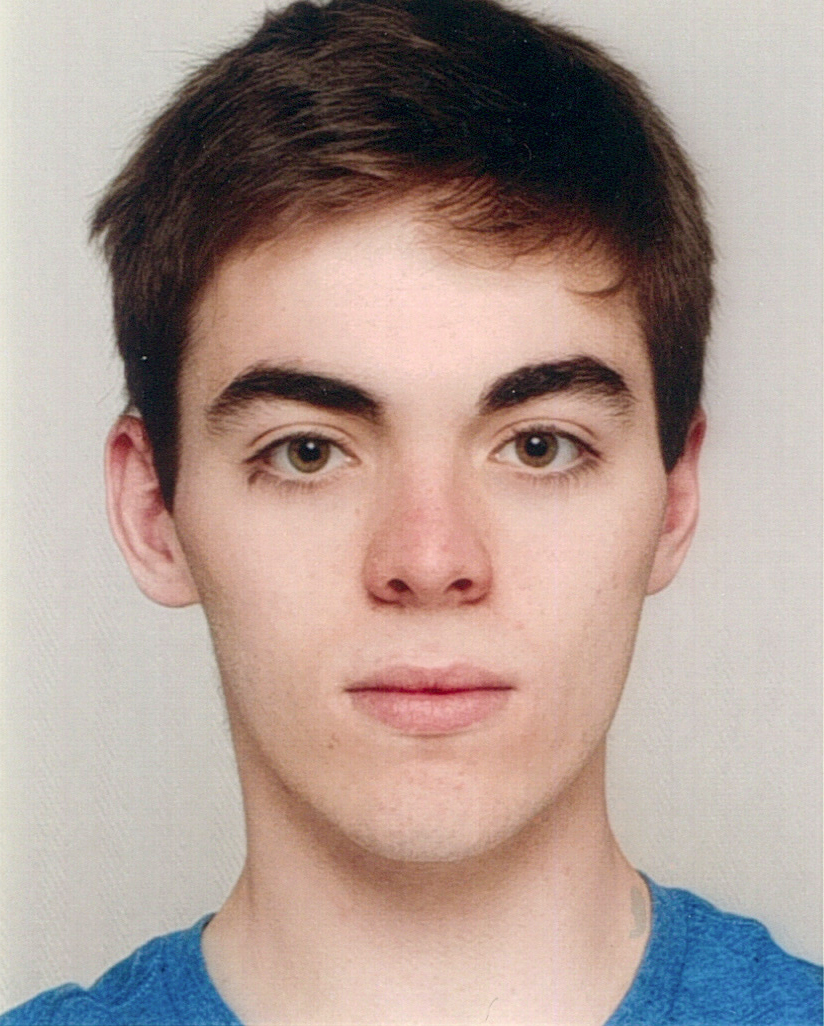
\includegraphics[scale=0.55]{images/clement_allain.jpg}
            \caption*{\footnotesize Clément \\ Allain}
        \end{subfigure}
        \begin{subfigure}{0.24\textwidth}
            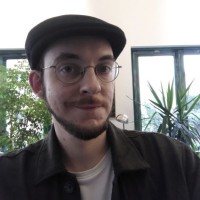
\includegraphics[scale=0.4]{images/basile_clement.jpg}
            \caption*{\footnotesize Basile \\ Clément}
        \end{subfigure}
        \begin{subfigure}{0.24\textwidth}
            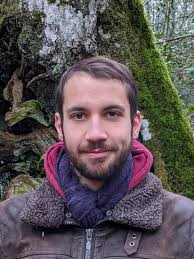
\includegraphics[scale=0.3]{images/alexandre_moine.jpg}
            \caption*{\footnotesize Alexandre \\ Moine}
        \end{subfigure}
        \begin{subfigure}{0.24\textwidth}
            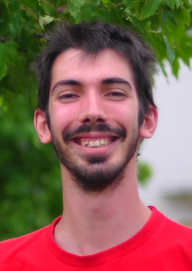
\includegraphics[scale=1.2]{images/gabriel_scherer.jpg}
            \caption*{\footnotesize Gabriel \\ Scherer}
        \end{subfigure}
        \caption*{The \Pstore team!}
    \end{figure}
\end{overbox}

\begin{overbox}<8>
    \begin{figure}
        \begin{subfigure}{0.4\textwidth}
            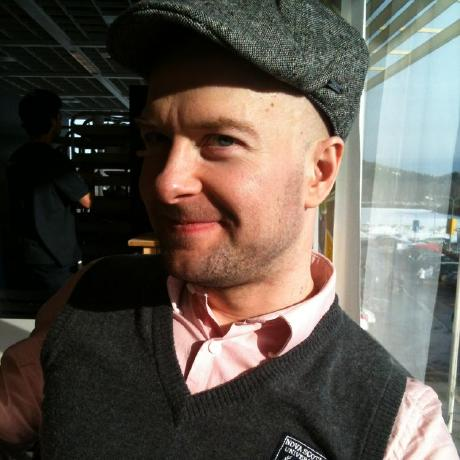
\includegraphics[scale=0.2]{images/vesa_karvonen.jpg}
            \caption*{\footnotesize Vesa Karvonen}
        \end{subfigure}
        \begin{subfigure}{0.4\textwidth}
            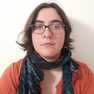
\includegraphics[scale=1]{images/carine_morel.jpg}
            \caption*{\footnotesize Carine Morel}
        \end{subfigure}
        \caption*{The \Saturn team!}
    \end{figure}
\end{overbox}

\begin{overbox}<11>
    \begin{figure}
        \begin{subfigure}{0.4\textwidth}
            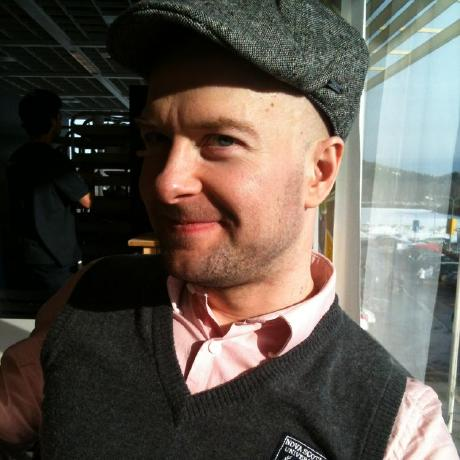
\includegraphics[scale=0.2]{images/vesa_karvonen.jpg}
            \caption*{\footnotesize Vesa Karvonen}
        \end{subfigure}
        \caption*{The main author of \Kcas!}
    \end{figure}
\end{overbox}

\only<12>{}

\end{adjustwidth}

\end{frame}

% ---------------------------------------------------------

\begin{frame}{\Zoo[]logy: why is it fun?}
Lockfree algorithms typically exhibit complex behaviors:
\begin{itemize}
    \item physical state $\neq$ logical state,
    \item external linearization points,
    \item future-dependent linearization points.
\end{itemize}
\vfill
\Iris is a good match for verifying them thanks to advanced mechanisms:
\begin{itemize}
    \item invariants to enforce protocols,
    \item atomic updates to materialize linearization points,
    \item prophecy variables to reason about the future.
\end{itemize}
\end{frame}
\section{Specimen \circled{1} : Michael-Scott queue}

\begin{frame}{Michael-Scott queue}
TODO
\end{frame}
\section{Specimen \circled{2} : \Kcas}

\begin{frame}{\Kcas}
TODO
\end{frame}

% ---------------------------------------------------------

\begin{frame}[plain, noframenumbering]
\LARGE
\begin{center}
	Thank you for your attention!
\end{center}
\end{frame}

% ---------------------------------------------------------

\end{document}
